

\tikzset{every picture/.style={line width=0.75pt}} %set default line width to 0.75pt        

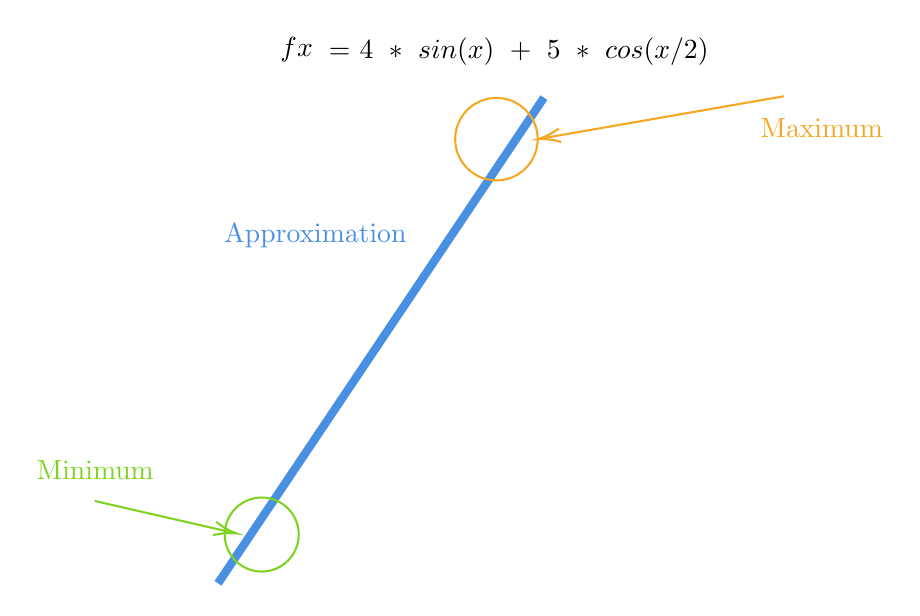
\begin{tikzpicture}[x=0.75pt,y=0.75pt,yscale=-1,xscale=1]
%uncomment if require: \path (0,300); %set diagram left start at 0, and has height of 300

% Plotting does not support converting to Tikz
%Straight Lines [id:da7392722993247356] 
\draw [color={rgb, 255:red, 74; green, 144; blue, 226 }  ,draw opacity=1 ][line width=3]    (365.13,49.33) -- (208.13,283.33) ;


%Straight Lines [id:da1413716903987703] 
\draw [color={rgb, 255:red, 126; green, 211; blue, 33 }  ,draw opacity=1 ]   (148.75,243.67) -- (215.18,258.89) ;
\draw [shift={(217.13,259.33)}, rotate = 192.9] [color={rgb, 255:red, 126; green, 211; blue, 33 }  ,draw opacity=1 ][line width=0.75]    (10.93,-3.29) .. controls (6.95,-1.4) and (3.31,-0.3) .. (0,0) .. controls (3.31,0.3) and (6.95,1.4) .. (10.93,3.29)   ;

%Straight Lines [id:da5550955277866936] 
\draw [color={rgb, 255:red, 245; green, 166; blue, 35 }  ,draw opacity=1 ]   (480.75,48.67) -- (364.1,68.99) ;
\draw [shift={(362.13,69.33)}, rotate = 350.12] [color={rgb, 255:red, 245; green, 166; blue, 35 }  ,draw opacity=1 ][line width=0.75]    (10.93,-3.29) .. controls (6.95,-1.4) and (3.31,-0.3) .. (0,0) .. controls (3.31,0.3) and (6.95,1.4) .. (10.93,3.29)   ;

%Shape: Circle [id:dp6334191871585448] 
\draw  [color={rgb, 255:red, 245; green, 166; blue, 35 }  ,draw opacity=1 ] (322.38,69.33) .. controls (322.38,58.36) and (331.28,49.46) .. (342.26,49.46) .. controls (353.23,49.46) and (362.13,58.36) .. (362.13,69.33) .. controls (362.13,80.31) and (353.23,89.21) .. (342.26,89.21) .. controls (331.28,89.21) and (322.38,80.31) .. (322.38,69.33) -- cycle ;
%Shape: Circle [id:dp9185427376772115] 
\draw  [color={rgb, 255:red, 126; green, 211; blue, 33 }  ,draw opacity=1 ] (211.33,259.83) .. controls (211.33,249.98) and (219.32,242) .. (229.17,242) .. controls (239.02,242) and (247,249.98) .. (247,259.83) .. controls (247,269.68) and (239.02,277.67) .. (229.17,277.67) .. controls (219.32,277.67) and (211.33,269.68) .. (211.33,259.83) -- cycle ;

% Text Node
\draw (246,26) node   {$fx$};
% Text Node
\draw (353,27) node  [align=left] {= $4\ *\ sin(x)\ +\ 5\ *\ cos(x/2)$};
% Text Node
\draw (149,229) node [color={rgb, 255:red, 126; green, 211; blue, 33 }  ,opacity=1 ] [align=left] {Minimum};
% Text Node
\draw (499,64) node [color={rgb, 255:red, 245; green, 166; blue, 35 }  ,opacity=1 ] [align=left] {Maximum};
% Text Node
\draw (255,116) node  [align=left] {\textcolor[rgb]{0.29,0.56,0.89}{Approximation}};


\end{tikzpicture}

